%%%%%%%%%%%%%%%%%%%%%%%%%%%%%%%%%%%%%%%%%%%%%%%%%
%       Microscopic analysis of load curve      %
%   Xavier                                      %
%%%%%%%%%%%%%%%%%%%%%%%%%%%%%%%%%%%%%%%%%%%%%%%%%

\subsection{Microscopic analysis of the load curve}
%Xavier
The sampling frequency used in the case of a microscopic analysis of the load curve is between 5 and 10k$Hz$. Such a frequency is required to access the transient responses of the devices. Using such a high sampling frequency is a way to avoid a difficulty encountered in macroscopic analysis coming from the fact that an appliance is generally switched on while other appliances are already in use. 
\\

An important point is that the transient response is linked with the physical role of the device. Studies have then been conducted to isolate characteristic parameters of the appliance from the transient response. Here is an example of a transient response :
\\
% Figure

\begin{figure}[H]
\centering
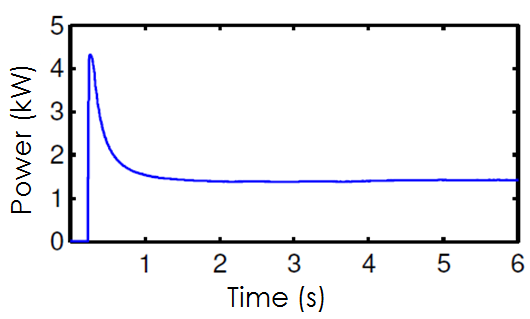
\includegraphics[scale=0.5]{figures/transient_response.png}
\caption{Transient response}
\label{fig:boxDescription}
\end{figure}



[2] address the problem of classification of transient signals which are modelled as a Smooth transition autoregressive model. Figure x shows some abrupt transitions on the transient signal, which are called breakpoints. Let $K$ denote the number of breakpoints, and $\underline{\tau} = [\tau_1,...,\tau_K]$ denote the sequence of the $K$ breakpoints. By convention, $[\tau_0;\tau_{K+1}]$ represents the observation interval of the signal. 
\\

 Therefore, the signal is modelled as a linear combination of regression functions $\{m_k\}_{k\in{1,K+1}}$.~$m_k$ is the regression model of the signal over the segment $[\tau_{k-1};\tau_{k}]$. Then, the signal is expressed as

\begin{equation}
\forall t\in [\tau_0;\tau_{K+1}],m(t)= \sum_{k=1}^{K+1}p_k(t)m_k(t)
\end{equation}

where $p_k(t)$ is the weight function of the $k^{th}$ regression model which can be expressed as follow
\begin{equation}
\forall k\in [1,K+1], p_k(t)= \pi_{\eta_{k-1}}(t-\tau_{k-1})-\pi_{\eta_{k}}(t-\tau_{k})
\end{equation}

$\pi_{\eta_{k}}$ is the transition function of the $k^{th}$ breakpoint, which depends on a vector of parameter $\eta_{k}$. In the model described in [1], $\pi_{\eta_{k}}$ is a sigmoide function, whose expression is 
\begin{equation}
\pi_{\eta_{k}} = \frac{1}{1+exp(\frac{t}{\lambda_k})}
\end{equation}

The only element in $\eta_{k}$ is then $\lambda_k$, which is a scale parameter. Let $\underline{\lambda}$ denote the concatenation of all the scale parameters $\underline{\lambda} = [\lambda_1,...,\lambda_K]$.
\\

 Regression model are considered in [2] as polynomial 

\begin{equation}
m_k(t)= \sum_{q=0}^{Q_k} \beta^{(q)} _kt^q
\end{equation}

$\beta^{(q)} _k$ is the $q^{th}$ order regression coefficient of the $k^{th}$ regression model, and $Q_k$ is the order of $m_k(t)$. As it was the case for $\lambda$, $\beta$ regroups all the $\beta_k$ coefficients and $Q$ all the $Q_k$ coefficients.
\\

A common model for the observed signal is 


\begin{equation}
s(t)=m(t) + \epsilon (t)
\end{equation}

$\epsilon (t)$ is an additive white Gaussian noise whose variance is $\sigma^2$. The different parameters which have to be evaluated are then :
\begin{equation}
\theta=\{\underline{\lambda},\underline{\tau},\underline{\beta},\underline{Q},\sigma ^2,K\}
\end{equation}
\\


The approach presented in [2] is a Bayesian one. The $posterior$ probability density function of $\theta$ is obtained thanks to the Bayes formula. The algorithm used to sample the distibution is a Reversible Jump Markov chain Monte Carlo (RJMCMC). The algorithm consists in a main loop which is repeated a high number of time. The higher the number of iterations, the more accurate the algorithm. A new set of values is purposed for $\theta$ during each iteration. The different kind of movements that can be purposed concerning $\theta$ are :
\begin{itemize}
\item Birth of a transition
\item Death of a transition
\item Division of an existing transition
\item Fusion of two existings transitions
\item Update of a transition
\end{itemize}
The movement is then accepted or rejected with a certain probability, which depends on Hasting-Green-Metropolis ratio. 
\\

The classification of electrical devices is then done thanks to $\theta$. Since that study was more a theoretical than a practical work, it has not been implemented yet on the box, but is functionnal for very basics signals.

